% PRTE notes: RTE with source term expressed via Green's function
\chapter{基于神经网络自编码器的含源项辐射输运求解}
\section{研究动机}
在之前章节中，我们介绍了基于神经网络自编码器的辐射传输方程（RTE）求解方法，重点关注了无源项的稳态问题。然而，在许多实际应用中，辐射传输过程往往伴随着体源项的存在，例如在核反应堆中中子源的分布、天体物理中的辐射源等。因此，扩展现有方法以处理含源项的RTE具有重要的理论意义和实际价值。

首先，我们介绍含源项的稳态辐射传输方程
\begin{equation}\label{eq:rte-source}
    (\bOmega\cdot\nabla + \mu_t(\br)) I(\br,\bOmega)
    - \frac{\mu_s(\br)}{S_{d-1}} \int_{\mathbb{S}^{d-1}} p(\bOmega,\bOmega^*) I(\br,\bOmega^*)\,\diff\bOmega^*
    = q(\br,\bOmega),
\end{equation}
其中 $\br\in D\subset\mathbb{R}^d$，$\bOmega\in\mathbb{S}^{d-1}$，$I(\br,\bOmega)$ 为辐射强度，$\mu_t(\br)=\mu_a(\br)+\mu_s(\br)$，散射核 $p(\bOmega,\bOmega^*)$ 满足角向归一化 $\frac{1}{S_{d-1}}\int_{\mathbb{S}^{d-1}} p(\bOmega,\bOmega^*)\diff\bOmega^*=1$，$q(\br,\bOmega)$ 为源项。

由于方程是线性的，可以采用格林函数思路：构造满足伴随方程的 $G(\br,\bOmega;\br',\bOmega')$ 后，将任意源项 $q(\br,\bOmega)$ 分解成位置-方向的脉冲源并线性叠加得到解的体积分表示。边界贡献同样可线性叠加；为突出体源部分并避免额外复杂度，这里先取齐次（零）边界作为基准解，若需非零边界条件，只需再叠加相应的边界响应即可。因此在本章节中，我们只考虑齐次边界条件下的含源项 RTE 求解。

传统的数值方法，如有限差分法、有限元法等，通常需要对源项进行离散化处理，并结合边界条件进行求解。然而，这些方法在处理复杂几何形状和高维问题时，计算成本较高且易受数值误差影响。近年来，神经网络方法在解决偏微分方程方面展现出强大的能力，特别是在高维问题中表现出色。在本章节中，我们通过引入自编码器结构来表示基函数，从而实现对含源项 RTE 的高效求解。

在之后的章节，我们将详细介绍基于神经网络自编码器的含源项 RTE 求解方法，包括解结构分析、网络设计以及训练策略等内容。通过这种方法，我们期望能够在保持高精度的同时，显著降低计算复杂度，为实际应用提供有效的数值工具。

\section{解结构简析}

考虑式~\eqref{eq:rte-source} 的含体源项稳态辐射传输方程
\begin{equation}
    (\bOmega\cdot\nabla + \mu_t(\br)) I(\br,\bOmega)
    - \frac{\mu_s(\br)}{S_{d-1}} \int_{\mathbb{S}^{d-1}} p(\bOmega,\bOmega^*) I(\br,\bOmega^*)\,\diff\bOmega^*
    = q(\br,\bOmega),
\end{equation}
其中各符号含义同式~\eqref{eq:rte-source}。为简洁起见，定义线性算子
\begin{equation}
    \mathcal{L}[I(\br,\bOmega)]
    = (\bOmega\cdot\nabla + \mu_t(\br)) I(\br,\bOmega)
    - \frac{\mu_s(\br)}{S_{d-1}} \int_{\mathbb{S}^{d-1}} p(\bOmega,\bOmega^*) I(\br,\bOmega^*)\,\diff\bOmega^*,
\end{equation}
则含源辐射传输方程写作
\begin{equation}
    \mathcal{L}[I(\br,\bOmega)] = q(\br,\bOmega),
\end{equation}
这是一个非齐次线性积分-微分方程。求解思路是把任意体源 $q$ 拆解为位置-方向脉冲源的叠加，并用格林函数的线性叠加性得到总响应。

首先，先用格林函数 $G(\br,\bOmega;\br',\bOmega')$ 乘原方程并在 $D\times\mathbb{S}^{d-1}$ 上积分，得到

\begin{equation}
    \int G\,\mathcal{L}[I]=\int G\,q.
\end{equation}

更具体地，记积分变量为 $(\br,\bOmega)$，并将 $(\br',\bOmega')$ 视为参数，有
\begin{equation}
    \int_{D}\int_{\mathbb{S}^{d-1}} G(\br,\bOmega;\br',\bOmega')\, \mathcal{L}[I(\br,\bOmega)]\diff\bOmega\diff\br
    = \int_{D}\int_{\mathbb{S}^{d-1}} G(\br,\bOmega;\br',\bOmega')\, q(\br,\bOmega)\diff\bOmega\diff\br.
\end{equation}

然后分部积分，并用散度定理把导数从 $I$ 转移到 $G$。其中关键是对流项 $G(\bOmega\cdot\nabla I)$：注意 $\bOmega$ 与 $\br$ 无关，利用乘积求导
\begin{equation}
    \bOmega\cdot\nabla\bigl(GI\bigr)=G\,(\bOmega\cdot\nabla I)+I\,(\bOmega\cdot\nabla G),
\end{equation}
从而在对 $\br$ 积分时有
\begin{equation}
    \begin{aligned}
        \int_{D}\int_{\mathbb{S}^{d-1}} G\,(\bOmega\cdot\nabla I)\diff\bOmega\diff\br
         & = \int_{D}\int_{\mathbb{S}^{d-1}} \bOmega\cdot\nabla(GI)\diff\bOmega\diff\br
        - \int_{D}\int_{\mathbb{S}^{d-1}} I\,(\bOmega\cdot\nabla G)\diff\bOmega\diff\br             \\
         & = \int_{D}\int_{\mathbb{S}^{d-1}} \nabla\cdot\bigl(\bOmega\,GI\bigr)\diff\bOmega\diff\br
        - \int_{D}\int_{\mathbb{S}^{d-1}} I\,(\bOmega\cdot\nabla G)\diff\bOmega\diff\br             \\
         & = \int_{\partial D}\int_{\mathbb{S}^{d-1}} (\bOmega\cdot\bn)\,G\,I\diff\bOmega\diff S
        - \int_{D}\int_{\mathbb{S}^{d-1}} I\,(\bOmega\cdot\nabla G)\diff\bOmega\diff\br,
    \end{aligned}
\end{equation}
最后一步即对向量场 $\bOmega\,GI$ 应用散度定理
\begin{equation}
    \int_{D}\nabla\cdot(\bOmega\,GI)\diff\br=\int_{\partial D}(\bOmega\cdot\bn)GI\diff S.
\end{equation}

将上述对流项的结果与吸收/散射项合并，并将体积分中的导数项移到 $G$ 一侧，即得到
\begin{equation}
    \int_{D}\int_{\mathbb{S}^{d-1}} G\, \mathcal{L}[I] \diff\bOmega\diff\br
    = \int_{D}\int_{\mathbb{S}^{d-1}} I\, \mathcal{L}^*[G] \diff\bOmega\diff\br
    + \int_{\partial D}\int_{\mathbb{S}^{d-1}} (\bOmega\cdot\bn)\, I\, G \diff\bOmega\diff S,
\end{equation}
其中 $D$ 为求解区域，$\partial D$ 为其边界，$\bn$ 为外法向。其中，伴随算子 $\mathcal{L}^*$ 定义为
\begin{equation}
    \mathcal{L}^*[G] = - (\bOmega\cdot\nabla) G + \mu_t(\br) G
    - \frac{\mu_s(\br)}{S_{d-1}} \int_{\mathbb{S}^{d-1}} p(\bOmega^*,\bOmega) G(\br,\bOmega^*;\br',\bOmega')\diff\bOmega^*.
\end{equation}

接下来，若$\mathcal{L}^*$满足脉冲源条件
\begin{equation}
    \mathcal{L}^*[G(\br,\bOmega;\br',\bOmega')] = \delta_{\{\br'\}}(\br)\,\delta(\bOmega-\bOmega'),
\end{equation}
其中 $\delta_{\{\br'\}}(\br)$ 与 $\delta(\bOmega-\bOmega')$ 分别表示空间（或边界）上的 Dirac 分布与角度空间中的 Dirac $\delta$ 函数，表示在源点 $(\br',\bOmega')$ 施加单位脉冲时，观测点 $(\br,\bOmega)$ 的辐射强度响应。将该条件代入第二步右端体积分中的 $\mathcal{L}^*[G]$，并利用 $\delta$ 的筛选性
\begin{equation}
    \int_{D}\int_{\mathbb{S}^{d-1}} I(\br,\bOmega)\,\delta_{\{\br'\}}(\br)\,\delta(\bOmega-\bOmega')\diff\bOmega\diff\br
    = I(\br',\bOmega'),
\end{equation}
即可将体积分项化为待求量在 $(\br',\bOmega')$ 处的取值。

将上述结果与第一步等式合并，可得到带边界项的中间恒等式
\begin{equation}
    \begin{aligned}
        I(\br',\bOmega')
         & + \int_{\partial D}\int_{\mathbb{S}^{d-1}} (\bOmega\cdot\bn)\, I(\br,\bOmega)\, G(\br,\bOmega;\br',\bOmega')\diff\bOmega\diff S \\
         & = \int_{D}\int_{\mathbb{S}^{d-1}} G(\br,\bOmega;\br',\bOmega')\, q(\br,\bOmega)\diff\bOmega\diff\br.
    \end{aligned}
\end{equation}

最后，将观测点记为 $(\br,\bOmega)$、源点记为 $(\br',\bOmega')$，得到含源 RTE 的格林函数积分解
\begin{equation}
    \begin{aligned}
        I(\br,\bOmega)
         & = \int_{D}\int_{\mathbb{S}^{d-1}} G(\br,\bOmega;\br',\bOmega')\, q(\br',\bOmega')\diff\bOmega'\diff\br'                                  \\
         & \quad - \int_{\partial D}\int_{\mathbb{S}^{d-1}} (\bOmega'\cdot\bn') I(\br',\bOmega') G(\br,\bOmega;\br',\bOmega')\diff\bOmega'\diff S'.
    \end{aligned}\label{eq:rte-green-source}
\end{equation}
散度定理将 $\bOmega\cdot\nabla$ 的体积分转化为边界积分，是伴随算子边界项的唯一来源。上式第一项对应体源的叠加贡献，第二项刻画边界入射或出射辐射的贡献；若边界无入射源（如真空或黑体），边界项为零，积分解仅保留体积分。

需要说明的是，在之前的章节我们已经介绍了无源项 RTE 的格林函数求解方法，也即~\eqref{eq:rte-green-source} 中的边界项部分。因此在后续章节中我们只考虑齐次边界条件下的含源项 RTE 求解，即
\begin{equation}
    I|_{\Gamma_{-}}(\br,\bOmega)                              = 0,
\end{equation}
其中 $\Gamma_{-}=\{(\br,\bOmega):\br\in\partial D, \bOmega\cdot\bn<0\}$。
如果是非齐次边界条件，只需将边界响应部分单独计算后与体源响应叠加即可。因此，~\eqref{eq:rte-green-source}可简化为
\begin{equation}
    I(\br,\bOmega)
    = \int_{D}\int_{\mathbb{S}^{d-1}} G(\br,\bOmega;\br',\bOmega')\, q(\br',\bOmega')\diff\bOmega'\diff\br'.
\end{equation}

\section{网络结构}
含源项RTE的格林函数积分解（齐次边界条件下）是网络结构设计的核心理论依据。本节首先通过公式推导明确源项-格林函数-解的线性映射关系，再基于该关系构建编码器-解码器自编码器框架，实现对含源项RTE解的高效近似。

\subsection{核心映射关系的公式推导}
现在我们的目标是设计神经网络结构，能够高效逼近含源项RTE的解映射关系。即求解算子$\mathcal{A}$，使得：
\begin{equation}
    \mathcal{A}: q(\br',\bOmega') \mapsto I(\br,\bOmega).
\end{equation}

齐次边界条件下含源项RTE的格林函数积分解为
\begin{equation}\label{eq:green-core}
    I(\br,\bOmega)
    = \int_{D}\int_{\mathbb{S}^{d-1}} G(\br,\bOmega;\br',\bOmega')\, q(\br',\bOmega')\diff\bOmega'\diff\br'.
\end{equation}

上式描述了源项 $q$ 经由格林函数 $G$ 映射为解 $I$。直接对该积分进行数值计算面临两大挑战：
\begin{enumerate}
    \item 高维灾难：空间维度 $d$ 与角度维度 $d-1$ 联合导致积分区域规模指数级增长；
    \item 格林函数无解析解：仅在极少数简单场景下可推导 $G$ 的解析表达式，复杂场景下只能依赖数值近似。
\end{enumerate}

为解决上述问题，我们引入基函数展开思想，对源项 $q$ 和格林函数 $G$ 进行统一基表示，将高维积分映射转化为低维线性组合运算。具体推导步骤如下：

\paragraph{步骤1：源项的基函数展开}
设存在 $K$ 个源域基函数 $\{\phi_k(\br',\bOmega')\}_{k=1}^K$，其张成的空间可近似任意体源项 $q(\br',\bOmega')$。则源项可展开为基函数的线性组合：
\begin{equation}\label{eq:q-expand}
    q(\br',\bOmega') \approx \sum_{k=1}^{K} q_k\, \phi_k(\br',\bOmega'),
\end{equation}
其中 $q_k$ 为源项在基函数上的展开系数，由源项与基函数的内积确定：
\begin{equation}\label{eq:q-coeff}
    q_k = \int_{D}\int_{\mathbb{S}^{d-1}} q(\br',\bOmega')\, \phi_k(\br',\bOmega')\,\diff\bOmega'\diff\br'.
\end{equation}
基函数数量 $K$ 远小于源域离散化点数，实现源项的降维表示。

\paragraph{步骤2：格林函数的基函数展开}
利用格林函数的线性响应特性，将其关于源域变量 $(\br',\bOmega')$ 基于同一组基函数 $\{\phi_k(\br',\bOmega')\}_{k=1}^K$ 展开：
\begin{equation}\label{eq:g-expand}
    G(\br,\bOmega;\br',\bOmega') \approx \sum_{k=1}^{K} G_k(\br,\bOmega)\, \phi_k(\br',\bOmega'),
\end{equation}
其中 $G_k(\br,\bOmega)$ 为格林函数的展开系数，仅与观测域变量 $(\br,\bOmega)$ 相关，刻画第 $k$ 个源域基函数对应的观测域响应。

\paragraph{步骤3：解的低维线性组合推导}
将\eqref{eq:q-expand}与\eqref{eq:g-expand}代入核心积分解\eqref{eq:green-core}，可得
\begin{equation}
    \begin{aligned}
        I(\br,\bOmega)
         & = \int_{D}\int_{\mathbb{S}^{d-1}} \left(\sum_{k_1=1}^{K} G_{k_1}(\br,\bOmega)\, \phi_{k_1}(\br',\bOmega')\right)
        \left(\sum_{k_2=1}^{K} q_{k_2}\, \phi_{k_2}(\br',\bOmega')\right)\diff\bOmega'\diff\br'                                                                                                                           \\
         & = \sum_{k_1=1}^{K}\sum_{k_2=1}^{K} G_{k_1}(\br,\bOmega)\, q_{k_2}\, \underbrace{\int_{D}\int_{\mathbb{S}^{d-1}} \phi_{k_1}(\br',\bOmega')\, \phi_{k_2}(\br',\bOmega')\, \diff\bOmega'\diff\br'}_{W_{k_1 k_2}}.
    \end{aligned}
\end{equation}
其中 $W_{k_1 k_2}$ 为基函数的Gram矩阵元素，仅与源域基函数有关，一旦基函数确定即可预先计算。

为简化表达式，定义系数向量
\begin{equation}
    \boldsymbol{G}(\br,\bOmega):=\bigl[G_k(\br,\bOmega)\bigr]_{k=1}^{K}, \quad
    \boldsymbol{q}:=\bigl[q_k\bigr]_{k=1}^{K},
\end{equation}
以及 Gram 矩阵 $\boldsymbol{W} = [W_{k_1 k_2}]_{K\times K}$，则解 $I(\br,\bOmega)$ 可简化为低维向量乘积形式：
\begin{equation}\label{eq:i-vector}
    I(\br,\bOmega) = \boldsymbol{G}(\br,\bOmega)^{\top} \boldsymbol{W} \boldsymbol{q}.
\end{equation}

\eqref{eq:i-vector} 是网络设计的核心理论支撑：只需通过神经网络学习源域基函数 $\{\phi_k\}$ 和观测域系数向量 $\boldsymbol{G}$，即可将高维积分求解转化为低维向量运算，显著降低计算复杂度。

\subsection{整体框架概述}
基于上述核心映射关系，我们设计端到端的神经网络自编码器框架，整体流程分为两个阶段：
\begin{enumerate}
    \item \textbf{编码器阶段}：学习最优基函数 $\{\phi_k^{\text{NN}}(\br',\bOmega')\}_{k=1}^K$，实现对任意体源项 $q$ 的低维重构；
    \item \textbf{解码器阶段}：学习格林函数的观测域系数向量 $\boldsymbol{G}^{\text{NN}}(\br,\bOmega)$，结合 Gram 矩阵 $\boldsymbol{W}$ 和源项系数 $\boldsymbol{q}$，实现对辐射强度 $I$ 的精准拟合。
\end{enumerate}

两个阶段通过 Gram 矩阵 $\boldsymbol{W}$ 实现关联，共同构成“源项输入-解输出”的端到端求解框架，在保持高精度的同时，显著降低高维问题的计算成本。

\subsection{编码器：学习源域基函数}\label{sec:prte-encoder}
编码器的核心任务是学习一组具有强重构能力的源域基函数 $\phi_k^{\text{NN}}(\br',\bOmega')\in\mathbb{R}$（上标 $\text{NN}$ 表示由神经网络学习得到）。

对于任意体源项 $q(\br',\bOmega')$，利用编码器学习到的 $K$ 个基函数，其展开形式为
\begin{equation}
    \begin{aligned}
        q(\br',\bOmega') & \approx \sum_{k=1}^{K} q_k\, \phi_k^{\text{NN}}(\br',\bOmega'),                                                 \\
        q_k              & = \int_{D}\int_{\mathbb{S}^{d-1}} q(\br',\bOmega')\, \phi_k^{\text{NN}}(\br',\bOmega')\,\diff\bOmega'\diff\br'.
    \end{aligned}
\end{equation}

这里我们使用一组全连接神经网络来表示基函数 $\phi_k^{\text{NN}}$。具体地，定义编码器网络如下，其输出为 $K$ 维向量：
\begin{equation}
    \text{Encoder}_{\boldsymbol{\theta}}(\br',\bOmega') = \bigl[\phi_k^{\text{NN}}(\br',\bOmega')\bigr]_{k=1}^{K},
\end{equation}
其中 $\boldsymbol{\theta}$ 为网络参数。

编码器的训练目标是最小化源项的重构误差。定义逐点重构损失函数
\begin{equation}
    \ell_\phi(\br',\bOmega') = \left| q(\br',\bOmega') - \sum_{k=1}^{K} q_k\, \phi_k^{\text{NN}}(\br',\bOmega') \right|.
\end{equation}
整体训练损失为逐点损失在源域上的积分（或离散化求和）：
\begin{equation}
    L_\phi = \int_{D}\int_{\mathbb{S}^{d-1}} \ell_\phi(\br',\bOmega')\diff\bOmega'\diff\br'.
\end{equation}
通过梯度下降算法最小化 $L_\phi$，即可得到最优源域基函数 $\{\phi_k^{\text{NN}}\}_{k=1}^K$。

\subsection{解码器：学习格林函数观测域系数}\label{sec:prte-decoder}
解码器的核心任务是学习格林函数的观测域系数向量 $\boldsymbol{G}^{\text{NN}}(\br,\bOmega)$，基于编码器的基函数和 Gram 矩阵，实现对辐射强度 $I$ 的精准拟合。

基于核心映射关系的推导，将格林函数关于源域变量 $(\br',\bOmega')$ 用编码器学习到的基函数展开：
\begin{equation}
    G(\br,\bOmega;\br',\bOmega') \approx \sum_{k=1}^{K} G_k^{\text{NN}}(\br,\bOmega)\, \phi_k^{\text{NN}}(\br',\bOmega').
\end{equation}
其中 $G_k^{\text{NN}}(\br,\bOmega)$ 为解码器输出的系数，仅依赖观测域变量。

结合编码器的源项系数 $\boldsymbol{q}$ 和 Gram 矩阵 $\boldsymbol{W}$，辐射强度的近似解为
\begin{equation}
    I(\br,\bOmega) = \boldsymbol{G}^{\text{NN}}(\br,\bOmega)^{\top} \boldsymbol{W} \boldsymbol{q},
\end{equation}
其中 $\boldsymbol{G}^{\text{NN}}(\br,\bOmega):=\bigl[G_k^{\text{NN}}(\br,\bOmega)\bigr]_{k=1}^{K}$。

现在需要确定解码器的网络结构。本文沿用DeepRTE的设计，使用衰减模块与散射模块来表示格林函数的观测域系数向量 $\boldsymbol{G}^{\text{NN}}(\br,\bOmega)$，对于维度不匹配的的问题，我们将散射模块最后的输出通过全连接层映射到 $K$ 维空间，得到最终的 $\boldsymbol{G}^{\text{NN}}$，即
\begin{equation}
    \boldsymbol{G}^{\text{NN}}(\br,\bOmega) = \text{Linear}\bigl(\text{GreenFunction}(\br,\bOmega, \br', \bOmega')\bigr),
\end{equation}
其中GreenFunction表示前述的衰减模块与散射模块的组合（具体过程见算法~\ref{alg:green-function}），Linear表示最后的全连接映射层。

解码器的训练目标是最小化辐射强度的拟合误差。定义逐点拟合损失函数
\begin{equation}
    \ell_G(\br,\bOmega) = \left| I_{\text{ref}}(\br,\bOmega) - \boldsymbol{G}^{\text{NN}}(\br,\bOmega)^{\top} \boldsymbol{W} \boldsymbol{q} \right|,
\end{equation}
其中 $I_{\text{ref}}(\br,\bOmega)$ 为传统数值方法得到的参考解（这里我们同样使用扫掠法）。

整体训练损失为逐点损失在观测域上的积分：
\begin{equation}
    L_G = \int_{D}\int_{\mathbb{S}^{d-1}} \ell_G(\br,\bOmega)\diff\bOmega\diff\br.
\end{equation}

\begin{enumerate}
    \item \textbf{预训练阶段}：单独训练编码器，得到基函数 $\{\phi_k^{\text{NN}}\}$ 并计算 Gram 矩阵 $\boldsymbol{W}$；
    \item \textbf{解码器训练阶段}：固定编码器参数和 $\boldsymbol{W}$，最小化 $L_G$ 得到 $\boldsymbol{G}^{\text{NN}}$；也可采用端到端联合训练，同时优化编码器和解码器参数；
    \item \textbf{推理阶段}：对新源项 $q_{\text{new}}$，先计算其系数 $\boldsymbol{q}_{\text{new}}$，再通过 $I_{\text{new}} = \boldsymbol{G}^{\text{NN}\top} \boldsymbol{W} \boldsymbol{q}_{\text{new}}$ 快速得到解。
\end{enumerate}

\section{实验设置}

本节考虑三维简化到二维的含源项稳态辐射输运问题，并仍采用扫掠法（sweeping）~\cite{adams2002fast} 生成训练与测试数据；相应实现可在 \href{https://github.com/mazhengcn/rte-dataset}{rte-dataset} 仓库复现。除以下两点外，本章所有实验设定均与上一章的数据集构造设置（见第~\ref{sec:dataset-construction} 节）保持一致：
\begin{enumerate}
    \item \textbf{边界条件}：采用齐次入射边界条件 $I\vert_{\Gamma_-}=0$；
    \item \textbf{源项}：引入体源 $q$，并使用零均值高斯随机场（Gaussian random field, GRF）在空间域 $D$ 上生成 $q(\br)$（在角度上取各向同性，即 $q(\br,\bOmega)=q(\br)$）。
\end{enumerate}

\subsection{高斯随机场}
我们采用基于频域功率谱的方式生成二维高斯随机场作为体源项 $q(\br)$~\cite{liu2019advances, ruan1998efficient}。该方法在离散网格上直接构造频域随机系数，再通过二维逆快速傅里叶变换（IFFT）得到物理空间的随机场；其中 $\alpha$ 控制随机场的平滑程度（$\alpha$ 越大，生成的场越平滑）。具体步骤如下。

首先，在与空间离散一致的 $N_{\text{mesh}}\times N_{\text{mesh}}$ 均匀网格上，利用 \texttt{fftfreq} 构造离散频率网格 $k_x,k_y$，并定义频率模平方与功率谱
\begin{equation}
    \begin{aligned}
        k^2(k_x,k_y)         & := k_x^2 + k_y^2,                        \\
        k^2(0,0)             & := 1,                                    \\
        \widehat{P}(k_x,k_y) & := \bigl(k^2(k_x,k_y)\bigr)^{-\alpha/2}, \\
        \widehat{P}(0,0)     & := 0.
    \end{aligned}
\end{equation}
其中将 $k^2(0,0)$ 置为 $1$ 仅用于避免 $\widehat{P}$ 的除零；随后令 $\widehat{P}(0,0)=0$ 等价于去除常数模态，从而避免生成的场带有整体偏置。

然后，逐点采样复高斯噪声
\begin{equation}
    \begin{aligned}
        \xi(k_x,k_y) & := a(k_x,k_y) + \mathrm{i}\,b(k_x,k_y),         \\
        a(k_x,k_y)   & \overset{\text{i.i.d.}}{\sim} \mathcal{N}(0,1), \\
        b(k_x,k_y)   & \overset{\text{i.i.d.}}{\sim} \mathcal{N}(0,1),
    \end{aligned}
\end{equation}
并将功率谱施加到随机系数上，再变换回物理空间
\begin{equation}
    \begin{aligned}
        \widehat{q}(k_x,k_y) & := \sqrt{\widehat{P}(k_x,k_y)}\,\xi(k_x,k_y),   \\
        q(\br)               & := \Re\bigl(\mathrm{IFFT}_2(\widehat{q})\bigr).
    \end{aligned}
\end{equation}

最后，为与代码实现一致，我们对 $q$ 做一次最小-最大归一化，将其缩放到 $[0,1]$ 区间用于训练：
\begin{equation}
    q \leftarrow \frac{q-\min(q)}{\max(q)-\min(q)}.
\end{equation}
表~\ref{tab:dataset_prte} 汇总了本章与上一章相比需要特别说明的条目以及其余沿用的超参数设置。

\begin{table}[!htp]
    \centering
    \begin{tabular}{lp{0.3\textwidth}ll}
        \toprule
        类别                      & 参数                     & 符号                      & 取值/范围                        \\ \midrule
        \multirow{2}{*}{空间区域}   & 计算区域                   & $D$                     & ${[0,1]}^2$                  \\
                                & 子区域                    & $D_\mu$                 & ${[0.4,0.6]}^2$              \\
        \midrule
        \multirow{4}{*}{截面系数}   & \multirow{2}{*}{总截面}   & \multirow{2}{*}{$\mut$} & $D_\mu$ 内：$\mathcal{U}(5,7)$ \\
                                &                        &                         & $D\backslash D_\mu$ 内：$10$   \\
                                & \multirow{2}{*}{散射截面}  & \multirow{2}{*}{$\mus$} & $D_\mu$ 内：$\mathcal{U}(2,4)$ \\
                                &                        &                         & $D\backslash D_\mu$ 内：$5$    \\
        \midrule
        \multirow{2}{*}{离散化}    & 空间网格点数                 & $N_{\text{mesh}}$       & 40                           \\
                                & 角度求积点数                 & $N_\text{quad}$         & 24                           \\ \midrule
        \multirow{1}{*}{边界条件}   & 入射边界条件                 & $I\vert_{\Gamma_-}$     & $0$（齐次）                      \\ \midrule
        \multirow{2}{*}{源项 $q$} & 频域功率谱指数（平滑度）           & $\alpha$                & $5.0$                        \\
                                & 归一化到 $[0,1]$           & ---                     & 是                            \\
        \midrule
        \multirow{3}{*}{散射参数}   & \multirow{3}{*}{不对称参数} & \multirow{3}{*}{$g$}    & $\mathcal{U}(0,0.2)$         \\
                                &                        &                         & $\mathcal{U}(0.4,0.6)$       \\
                                &                        &                         & $\mathcal{U}(0.7,0.9)$       \\
        \bottomrule
    \end{tabular}
    \bicaption{本章数据集构造与上一章的设定对比。}{Summary of dataset settings for this chapter (differences from Sec.~\ref{sec:dataset-construction}).}\label{tab:dataset_prte}
\end{table}

\subsection{网络参数设置}

表~\ref{tab:training_details_prte} 汇总了本章模型训练的超参数设置。关键参数在于基函数个数 $128$，以及基函数的隐藏层神经元数为 $256$。

\begin{table}[!htp]
    \centering
    \begin{tabular}{ll}
        \toprule
        超参数                                     & 取值                         \\ \midrule
        优化器（Optimizer）                          & Adam                       \\
        学习率策略（Schedule）                         & 余弦衰减（cosine decay）         \\
        学习率（Learning rate）                      & $1 \times 10^{-3}$         \\
        批大小（Global batch size）                  & 8                          \\
        配点数量（Collocation points） $N_\text{col}$ & 2048                       \\
        训练步数（Training steps）                    & 3,000,001                  \\
        基函数个数                                   & $128$                      \\
        基函数编码器隐藏层神经元数                           & 256                        \\
        基函数编码器层数                                & 4                          \\
        硬件                                      & 4$\times$ NVIDIA 4090 GPUs \\
        \bottomrule
    \end{tabular}
    \bicaption{模型训练超参数汇总。}{Summary of model training hyperparameters.}
    \label{tab:training_details_prte}
\end{table}


\section{数值实验}

为了验证基于神经网络自编码器的含源项辐射传输方程（RTE）求解方法的有效性和准确性，我们设计了一系列数值实验。


\subsection{编码器准确率评估}

本小节用于评估编码器学习到的源域基函数在体源项重构任务中的表现。模型在随机生成的 $1000$ 个源项 $q$上训练，并在编码器学习到的 $K$ 个基函数上计算其展开系数向量 $\boldsymbol{q}:=[q_k]_{k=1}^{K}$（其中 $K=128$）。随后，利用这些系数与基函数得到重构源项
\begin{equation}
    q^{\text{rec}}(\br)=\sum_{k=1}^{K} q_k\,\phi_k^{\text{NN}}(\br),
\end{equation}
并将 $q^{\text{rec}}$ 与原始源项 $q$ 进行对比（重构形式推导和loss计算格式见第~\ref{sec:prte-encoder} 节）。在训练完成之后，我们在和训练集同分布的$100$条测试集上进行测试（每个散射区间各100条），表~\ref{tab:accuracy_prte} 汇总了编码器在三种散射区间下的重构精度指标。可以看到，编码器在所有散射区间均表现出较低的均方误差（MSE）和均方根百分比误差（RMSPE），表明其学习到的基函数能够有效捕捉体源项的主要特征，实现高质量的重构。

\begin{figure}[!htp]
    \centering
    \begin{subfigure}[t]{0.32\textwidth}
        \centering
        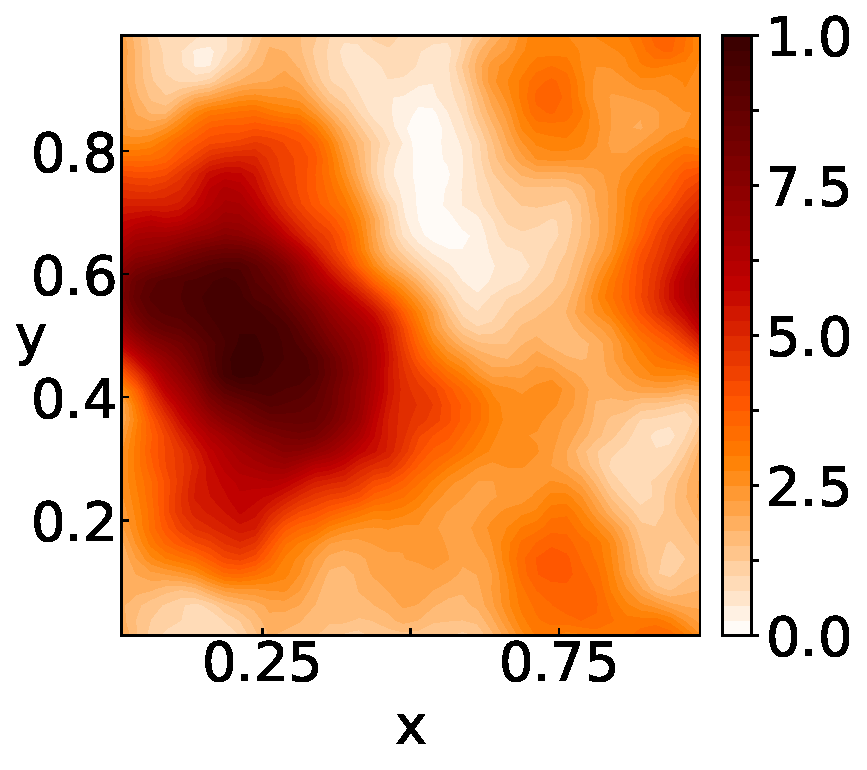
\includegraphics[width=\linewidth]{figures/autoencoder_label.pdf}
        \caption{$q_{\text{label}}$}
    \end{subfigure}\hfill
    \begin{subfigure}[t]{0.32\textwidth}
        \centering
        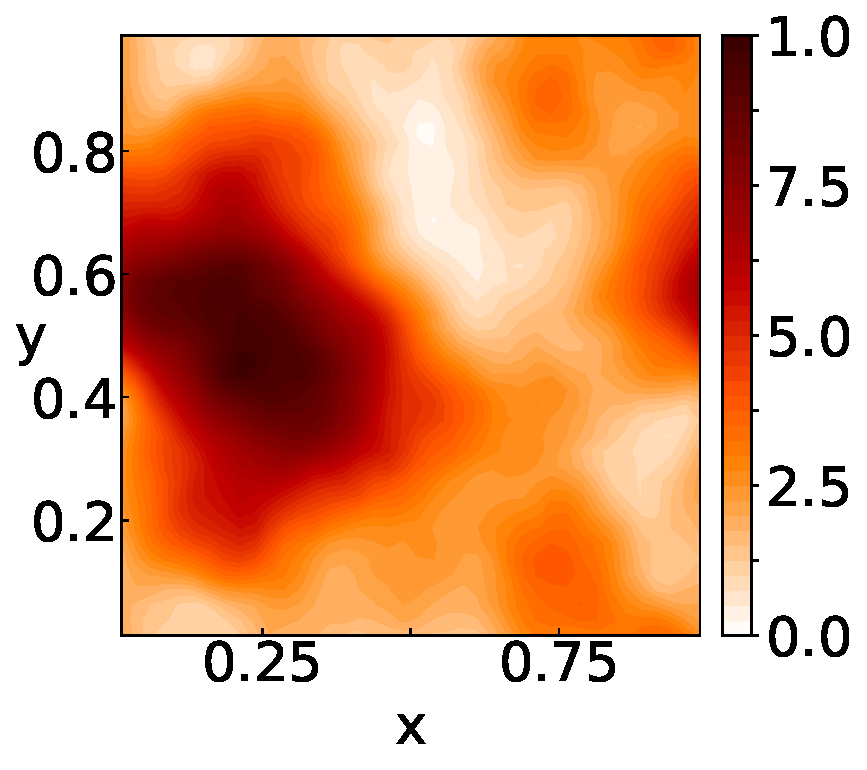
\includegraphics[width=\linewidth]{figures/autoencoder_pre.pdf}
        \caption{$q_{\text{predict}}$}
    \end{subfigure}\hfill
    \begin{subfigure}[t]{0.32\textwidth}
        \centering
        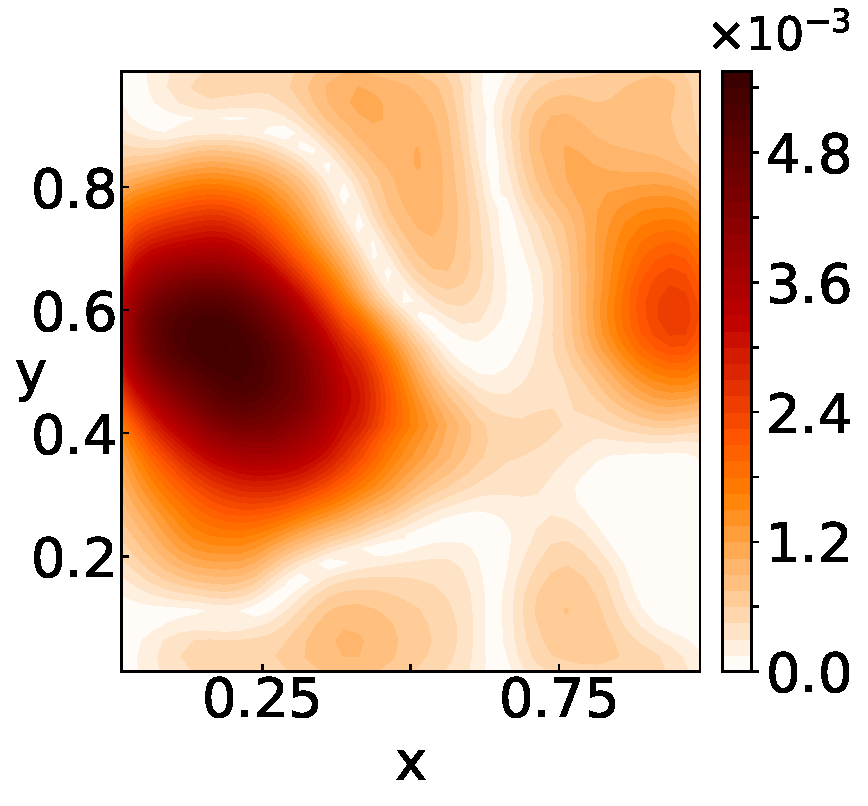
\includegraphics[width=\linewidth]{figures/autoencoder_error.pdf}
        \caption{Absolute error}
    \end{subfigure}
    \bicaption{在 $g\in (0,0.2)$ 情形下编码器的预测结果与真值比较。预测解的RMSPE为2.750\%}{Comparison between prediction and reference at $g\in(0,0.2)$ (RMSPE: 2.750\%).}
    \label{fig:autoencoder_example}
\end{figure}

\begin{table}[!htp]
    \centering
    \begin{tabular}{@{}cccccc@{}}
        \toprule
        模型                   & 参数量                     & 散射区间   & $g$ 取值范围   & MSE                  & RMSPE (\%) \\ \midrule
        \multirow{3}{*}{编码器} & \multirow{3}{*}{165760} & 近各向同性  & (0, 0.2)   & $6.03\times 10^{-4}$ & 4.894      \\ \cmidrule(l){3-6}
                             &                         & 中度各向异性 & (0.4, 0.6) & $7.11\times 10^{-4}$ & 5.214      \\ \cmidrule(l){3-6}
                             &                         & 强前向散射  & (0.7, 0.9) & $8.99\times 10^{-4}$ & 5.671      \\ \bottomrule
    \end{tabular}
    \bicaption{编码器在三种散射区间上的精度指标。}{Accuracy validation of autoencoder across three distinct scattering regimes.}\label{tab:accuracy_prte}
\end{table}

\subsection{解码器准确度评估}

本小节用于评估解码器在含源项 RTE 求解任务中的表现。我们随机生成 $1000$ 个源项 $q$和对应的辐射强度$I$做训练集，并利用编码器学习到的基函数计算Gram 矩阵 $\boldsymbol{W}$。随后，利用解码器学习到的格林函数观测域系数向量 $\boldsymbol{G}^{\text{NN}}(\br,\bOmega)$ 来重构辐射强度$I$（具体流程可参考~\ref{sec:prte-decoder}）。

表~\ref{tab:accuracy_prte_decoder} 汇总了解码器在三种散射区间（近各向同性、中度各向异性、强前向散射）下的精度指标。可以看到，当 $g\in(0,0.2)$ 时，解码器的 MSE 为 $9.46\times 10^{-5}$、RMSPE 为 3.163\%；当散射各向异性增强到 $g\in(0.4,0.6)$ 与 $g\in(0.7,0.9)$ 时，MSE 分别为 $1.04\times 10^{-4}$ 与 $1.52\times 10^{-4}$，RMSPE 分别为 3.280\% 与 3.612\%。整体而言，误差随前向散射增强略有上升，但三种区间的误差水平均维持在较低水平，说明解码器能够稳定地从源项系数重构辐射强度场，较好地捕捉含源项 RTE 解的主要结构并实现高质量拟合。

\begin{table}[!htp]
    \centering
    \begin{tabular}{@{}cccccc@{}}
        \toprule
        模型                   & 参数量                     & 散射区间   & $g$ 取值范围   & MSE                  & RMSPE (\%) \\ \midrule
        \multirow{3}{*}{解码器} & \multirow{3}{*}{268352} & 近各向同性  & (0, 0.2)   & $9.46\times 10^{-5}$ & 3.163      \\ \cmidrule(l){3-6}
                             &                         & 中度各向异性 & (0.4, 0.6) & $1.04\times 10^{-4}$ & 3.280      \\ \cmidrule(l){3-6}
                             &                         & 强前向散射  & (0.7, 0.9) & $1.52\times 10^{-4}$ & 3.612      \\ \bottomrule
    \end{tabular}
    \bicaption{解码器在三种散射区间上的精度指标。}{Accuracy validation of decoder across three distinct scattering regimes.}\label{tab:accuracy_prte_decoder}
\end{table}

\begin{figure}[!htp]
    \centering
    \begin{subfigure}[t]{0.32\textwidth}
        \centering
        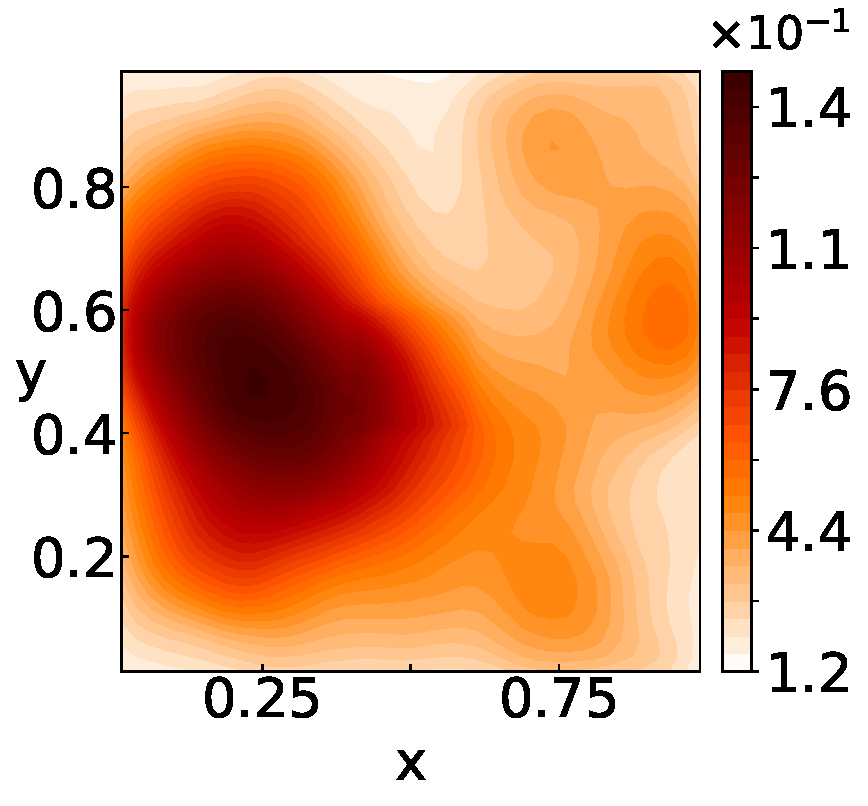
\includegraphics[width=\linewidth]{figures/decoder_label.pdf}
        \caption{$q_{\text{label}}$}
    \end{subfigure}\hfill
    \begin{subfigure}[t]{0.32\textwidth}
        \centering
        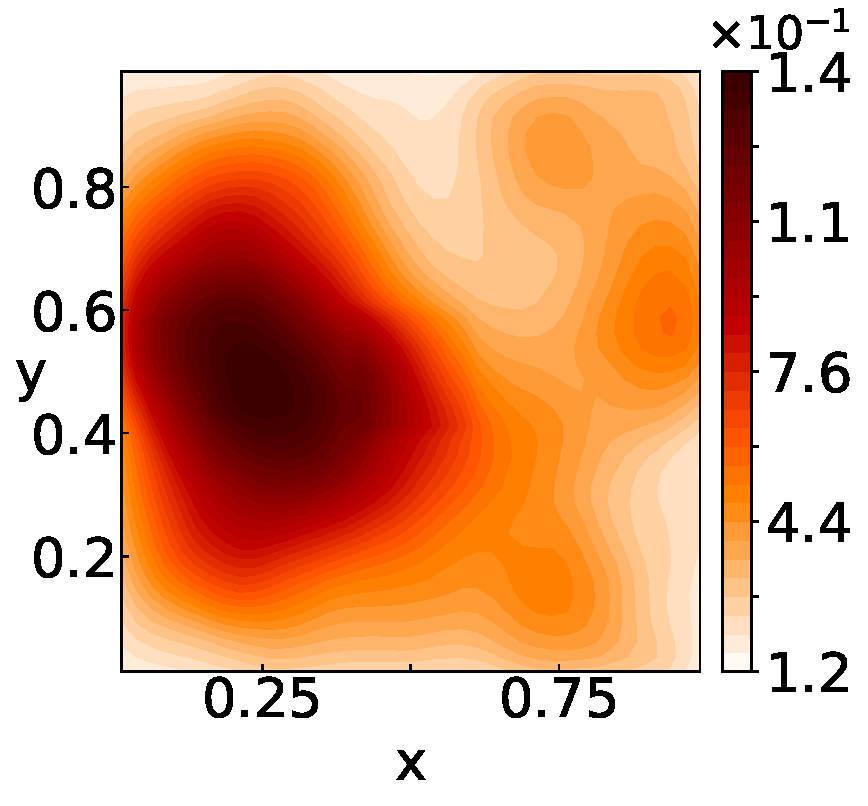
\includegraphics[width=\linewidth]{figures/decoder_pre.pdf}
        \caption{$q_{\text{predict}}$}
    \end{subfigure}\hfill
    \begin{subfigure}[t]{0.32\textwidth}
        \centering
        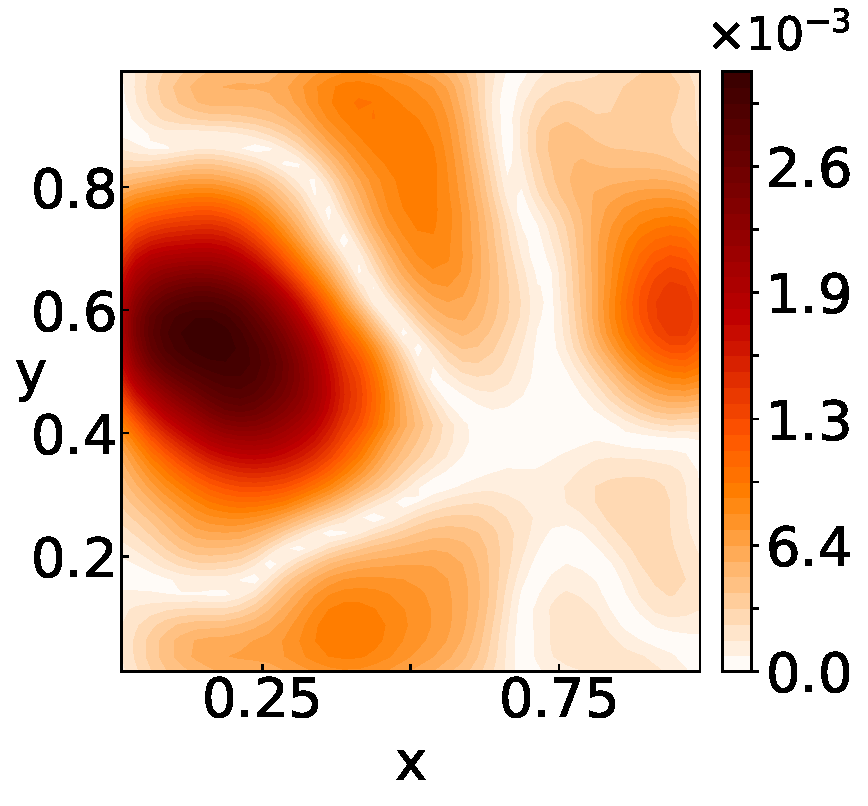
\includegraphics[width=\linewidth]{figures/decoder_error.pdf}
        \caption{Absolute error}
    \end{subfigure}
    \bicaption{在 $g\in (0,0.2)$ 情形下解码器的预测结果与真值比较。预测解的RMSPE为3.280\%}{Comparison between prediction and reference at $g\in(0,0.2)$ (RMSPE: 3.280\%).}
    \label{fig:decoder_example}
\end{figure}
